\documentclass[11pt]{article}

\usepackage[margin=1in]{geometry}
\usepackage{booktabs}
\usepackage{graphicx}
\usepackage{amsmath}
\usepackage{amssymb}
\usepackage{natbib}
\usepackage[hidelinks]{hyperref}
\usepackage{microtype}
\usepackage{array}
\usepackage{caption}
\usepackage{xcolor}

\bibliographystyle{plainnat}

\usepackage{setspace}
\onehalfspacing
\setlength{\parskip}{0.6\baselineskip}
\setlength{\parindent}{0pt}

\newcommand{\ind}[1]{\textsc{#1}}
\newcommand{\prtxt}{\mathrm{PR}}

\title{\textbf{When Do Attention Circuits Form?\\
Developmental Trajectories of Capability and Attention-Sink
Emergence Across Three 1B-Class Architectures}}

\author{Yongzhong Xu}

\date{}

\begin{document}

\maketitle

\begin{abstract}
\noindent
We track the developmental trajectory of attention-head circuit formation
across three 1B-class language models that span two architecture families
(dense transformer, mixture-of-experts) and two pretraining corpora
(The Pile, DCLM): Pythia 1B, OLMo 1B-0724-hf, and OLMoE 1B-7B-0924. At
each of 10 log-spaced revisions per model --- 30 mechanistic-interpretability
runs in total --- we apply a participation-ratio (PR) spectral signal and an
all-head capability-specific selectivity screen to identify induction,
previous-token, and BOS-attractor heads as they emerge.

Five findings. \textbf{(F1)} Layers 0 and 1 produce zero BOS-classified heads
at every revision in every model: the L0/L1 zero-BOS floor is an architectural
property, not a learned outcome. \textbf{(F2)} The whole-model BOS-attractor
fraction follows three distinct emergence shapes --- a gradual ramp in Pythia
1B (Pile, dense), a sharp phase transition in OLMo 1B (DCLM, dense, jumping
from 7\% to 70\% between adjacent checkpoints), and a gradual ramp in OLMoE
1B-7B (DCLM, MoE). \textbf{(F3)} In DCLM models, induction-circuit formation
precedes BOS-attractor formation by 10--20$\times$ in tokens (OLMo: induction
at 23B, BOS-50\% at 264B; OLMoE: induction at 20B, BOS-50\% at 419B).
Capability-circuit formation and attention-sink formation are two transitions,
not one. \textbf{(F4)} The capability-specific screen converges to the final
induction circuit within 0.3--2\% of total training tokens. Circuit
identification does not require the final model. \textbf{(F5)} For every
final-checkpoint induction head sampled across all three models, per-head PR
is elevated \emph{at or before} the first revision at which that head crosses
its capability-selectivity threshold.

The results refine the ``induction phase transition'' framing
\citep{olsson2022}: in 1B-class models trained on DCLM, the induction
transition and the attention-sink transition are separated by an order of
magnitude in tokens, and they have qualitatively different emergence shapes.
The L0/L1 zero-BOS floor and the data $\times$ architecture interaction in
BOS-attractor dynamics are constraints any mechanistic theory of attention
sinks must explain. We position this paper as the activation-space half of
an emergence story whose parameter-space half is studied in the SED/LCH
program \citep{xu2026sed,xu2026lch}.
\end{abstract}

\section{Introduction}

\citet{olsson2022} identified induction heads --- attention heads
implementing the $A\,B\,\ldots\,A\to B$ copy pattern --- as a key
mechanistic feature of in-context learning in transformer language models,
and connected their formation to a sharp ``phase transition'' visible as a
bump in the loss curve during pretraining. \citet{xiao2024} described a
distinct empirical phenomenon: pretrained LMs reliably allocate large
attention probability to the first (BOS) token regardless of content, a
behaviour they termed an \emph{attention sink}, which can be exploited for
KV-cache compression during streaming inference. Both phenomena are
described in terms of attention patterns; both are observed in modern
decoder-only language models; and both are sometimes folded together under
the heading of ``attention emergence during pretraining.''

This paper asks: when, exactly, do these two phenomena form during training
of 1B-class language models, and are they the \emph{same} transition? We
answer this empirically by tracking capability circuits (induction,
previous-token) and the BOS attractor side-by-side across three 1B-class
models that span two architecture families and two pretraining corpora.

\paragraph{Models.} Pythia 1B \citep{biderman2023}, a GPT-NeoX dense
transformer trained on The Pile \citep{gao2020pile}; OLMo 1B-0724-hf
\citep{groeneveld2024}, a Llama-style dense transformer trained on DCLM
\citep{li2024dclm}; and OLMoE 1B-7B-0924 \citep{muennighoff2024}, a
Llama-style mixture-of-experts transformer (1B active / 7B total
parameters, 64 experts, top-8 routing) trained on DCLM. These three models
factorize cleanly: Pythia vs OLMo isolates the corpus (Pile vs DCLM) at
fixed scale and dense architecture; OLMo vs OLMoE isolates the architecture
(dense vs MoE) at fixed corpus.

\paragraph{Method.} For each model we use the three-step recipe of the
companion methodology paper \citep{paper1_methodology}: per-head
participation ratio computed on a synthetic induction batch, an all-head
capability-specific selectivity screen, and group ablation. We apply the
screen at 10 log-spaced revisions per model --- 30 runs in total ---
producing a developmental panel.

\paragraph{Findings.} Five findings emerge, summarised in the abstract.
The central result is that in DCLM-trained 1B models, the induction
transition (Olsson's phenomenon) and the BOS-attractor transition
(Xiao's phenomenon) are separated by 10--20$\times$ in tokens and have
different emergence shapes (gradual ramp vs sharp jump). The two
phenomena cannot be identified with a single phase-transition event at
1B scale on DCLM data.

\paragraph{Position.} This paper is the \emph{activation-space} half of a
broader study of emergence in pretraining. The companion methodology paper
\citep{paper1_methodology} defines the recipe and validates it at the
final checkpoint; this paper applies the recipe developmentally; the
companion pattern-selectivity paper \citep{paper3_circuits} studies
cross-task generalisation. A complementary parameter-space program ---
spectral emergence dynamics (SED, \citealp{xu2026sed}) and the local
curvature hypothesis (LCH, \citealp{xu2026lch}) --- studies the same
emergence event in weight-space rather than activation-space. We return to
the bridge between these two windows in the Discussion.

\section{Related Work}

\paragraph{Induction heads and the phase transition.}
\citet{olsson2022} introduced the induction-head abstraction and reported a
``phase transition'' in pretraining co-located with a bump in the loss
curve, a sudden growth in in-context-learning capability, and the
appearance of attention heads implementing the prefix-match-and-copy
pattern. Their analysis used integrated-gradients-style attribution on
small ($\le\!\!100\mathrm{M}$-parameter) decoder-only models. The induction
phase transition has since become a standard reference point for
emergence-during-pretraining claims. This paper revisits the
\emph{transition} part of that claim at 1B scale across data and
architecture.

\paragraph{Attention sinks.}
\citet{xiao2024} documented attention sinks --- the observation that
trained decoder-only LMs reliably attend to the first token regardless of
content --- and used the phenomenon as a substrate for streaming inference
via fixed first-token KV retention. They did not study the formation
dynamics of sinks during pretraining. We do: BOS-attractor heads are
identified by the same selectivity screen as capability circuits, and
their per-revision counts give a token-resolved formation curve.

\paragraph{Pythia, OLMo, OLMoE.}
\citet{biderman2023} released Pythia precisely to enable cross-checkpoint
analyses of pretraining dynamics, with 154 checkpoints per model size
spanning random-init to 300B tokens. \citet{groeneveld2024} and
\citet{muennighoff2024} released OLMo and OLMoE with similar checkpoint
discipline. The 30-revision panel in this paper depends on all three
projects' checkpoint releases. We document checkpoint-availability
limitations (OLMo's earliest is 2B tokens; OLMoE's is 20B tokens) and
their effect on the resolved developmental curve in Section~\ref{sec:setup}.

\paragraph{Cross-architecture mechanistic transfer.}
Prior work has documented that the specific circuits a model uses for a
given task differ across architectures and scales
\citep{lieberum2023,wang2022ioi,marks2024sparse}. The cross-architecture
result in this paper is different: we hold the synthetic capability fixed
(induction on a controlled batch) and ask whether the \emph{timing} of
circuit formation, and the timing of the co-occurring BOS-attractor
phenomenon, transfer across pretraining corpora and architectures.

\paragraph{Automated circuit discovery.}
\citet{conmy2023} introduced ACDC, an iterative edge-pruning algorithm for
post-hoc circuit identification. The recipe used here is complementary and
predates a fully-trained model: a spectral signal that can be read at any
intermediate checkpoint, plus a per-class selectivity screen. We use ACDC
as motivation for the design rather than as a baseline.

\paragraph{Parameter-space emergence: SED and LCH.}
The SED \citep{xu2026sed} and LCH \citep{xu2026lch} papers study the same
emergence event from a different vantage point: the singular-value
geometry of weight matrices, and the local curvature of the loss surface.
Our PR signal is computed on activations, not parameters; the parameter-side
work treats the parameter spectrum of the same checkpoints. We discuss in
Section~\ref{sec:discussion} what an integrated account might look like.

\section{Methodology Recap}
\label{sec:method}

The recipe is defined in detail in \citet{paper1_methodology}. We summarise
here only what is needed to interpret the developmental results.

\paragraph{Synthetic induction batch.} 2000 sequences of length 256, RNG
seed 42. Each sequence has the structure $[\text{filler}]\,A\,B\,
[\text{filler}]\,A$, with $A$ and $B$ random tokens drawn from vocabulary
IDs $[100,\,10{,}000)$. The induction prediction is $B$ at the position
immediately following the second occurrence of $A$.

\paragraph{Per-head participation ratio.} For each (layer $L$, head $H$,
revision $t$), extract the per-head attention output at the second-$A$
position over the batch, giving $M \in \mathbb{R}^{N \times d_\text{head}}$
(here $N=2000$). Compute the singular spectrum $\{\sigma_i\}$ of $M$ and
the participation ratio
\[
  \prtxt(L,H,t) \;=\; \exp\!\big(H(p)\big),
  \quad p_i = \sigma_i^2 / \textstyle\sum_j \sigma_j^2,
\]
where $H(p)=-\sum_i p_i \log p_i$. The trajectory feature is the integral
$I(L,H) = \sum_t \max(\prtxt(L,H,t)-1,\,0)\cdot\Delta \log(\text{tokens}_t)$.
Throughout this paper we plot per-revision $\max(\prtxt(L,H,t)-1,0)$ as the
\emph{integrand} of $I$, so that temporal structure is preserved.

\paragraph{Capability-pattern screen.} For each head, compute attention
from the query position to canonical target positions for six classes:
\textsc{induction}, \textsc{previous-token}, \textsc{duplicate-token},
\textsc{first-token / bos}, \textsc{self}, and \textsc{local}. Selectivity
is (target attention)/(uniform-other baseline). A head is classified into
the class with maximum selectivity if that maximum exceeds 30$\times$
(class assignment); it is admitted to a class circuit if selectivity for
that class exceeds 50$\times$ (induction, BOS) or 100$\times$
(previous-token).

\paragraph{All-head capability-specific screen.} In the
attention-sink-dominated regime ($\ge\!70\%$ of heads classify as
\textsc{first-token} at the assignment threshold; see Section~\ref{sec:f2}),
ranking by best class surfaces BOS-attractor heads ahead of capability
heads. For circuit identification of a specific target capability $X$, we
instead take all heads with $\mathrm{sel}_X \ge \tau_X$ regardless of best
class. This is the screen used for the per-revision induction-circuit
identification in Sections~\ref{sec:f3}, \ref{sec:f4}, and~\ref{sec:f5}.

\paragraph{Causal verification.} Group-ablate the screen-identified circuit
by zeroing the per-head slice of the residual contribution at the attention
output projection. Matched-random controls share layers and head count but
not identities. Top-1 accuracy on the synthetic induction batch is the
primary metric. Final-checkpoint circuit ablations are documented in the
companion methodology paper and not repeated here; this paper focuses on
the per-revision trajectory.

\section{Setup: a 30-Revision Developmental Panel}
\label{sec:setup}

We run the spectral-and-screen recipe at 10 log-spaced revisions in each
of the three 1B-class models, for 30 mechanistic-interpretability runs in
total.

\paragraph{Revision schedules.} Pythia 1B's checkpoint set spans
\texttt{step1} ($\approx 2{\times}10^6$ tokens, essentially random
initialisation) through \texttt{step143000} ($\approx 300\mathrm{B}$
tokens, end of training). OLMo 1B's set spans
\texttt{step1000} (2B tokens) through
\texttt{step1454000} (3048B tokens). OLMoE 1B-7B's set spans
\texttt{step5000} (20B tokens) through \texttt{step1223842}
(5117B tokens). The
selected log-spaced revisions for each model are listed in
Table~\ref{tab:revisions}.

\begin{table}[t]
\centering
\caption{Revisions used for the 30-run developmental panel.
``Tokens'' is the cumulative training-token count published on the
respective HuggingFace model card; ``frac'' is tokens divided by the
model's final training-token count.}
\label{tab:revisions}
\small
\begin{tabular}{l r r r}
\toprule
Model & Revision label & Tokens (approx.) & frac of training \\
\midrule
Pythia 1B           & \texttt{step1}      & $2.1\,\mathrm{M}$    & $7\times10^{-6}$ \\
                    & \texttt{step8}      & $8.4\,\mathrm{M}$    & $3\times10^{-5}$ \\
                    & \texttt{step64}     & $6.7\times10^{7}$    & $2\times10^{-4}$ \\
                    & \texttt{step256}    & $5.4\times10^{8}$    & $2\times10^{-3}$ \\
                    & \texttt{step512}    & $1.1\,\mathrm{B}$    & $4\times10^{-3}$ \\
                    & \texttt{step3000}   & $6.3\,\mathrm{B}$    & $2\times10^{-2}$ \\
                    & \texttt{step10000}  & $21\,\mathrm{B}$     & $7\times10^{-2}$ \\
                    & \texttt{step38000}  & $80\,\mathrm{B}$     & $2.7\times10^{-1}$ \\
                    & \texttt{step143000} & $300\,\mathrm{B}$    & $1.0$ \\
\midrule
OLMo 1B             & \texttt{step1000}    & $2\,\mathrm{B}$      & $7\times10^{-4}$ \\
                    & \texttt{step5000}    & $10\,\mathrm{B}$     & $3\times10^{-3}$ \\
                    & \texttt{step11000}   & $23\,\mathrm{B}$     & $8\times10^{-3}$ \\
                    & \texttt{step25000}   & $52\,\mathrm{B}$     & $1.7\times10^{-2}$ \\
                    & \texttt{step56000}   & $117\,\mathrm{B}$    & $3.8\times10^{-2}$ \\
                    & \texttt{step126000}  & $264\,\mathrm{B}$    & $8.7\times10^{-2}$ \\
                    & \texttt{step312000}  & $654\,\mathrm{B}$    & $2.1\times10^{-1}$ \\
                    & \texttt{step644000}  & $1350\,\mathrm{B}$   & $4.4\times10^{-1}$ \\
                    & \texttt{step1454000} & $3048\,\mathrm{B}$   & $1.0$ \\
\midrule
OLMoE 1B-7B         & \texttt{step5000}    & $20\,\mathrm{B}$     & $3.9\times10^{-3}$ \\
                    & \texttt{step10000}   & $41\,\mathrm{B}$     & $8.0\times10^{-3}$ \\
                    & \texttt{step25000}   & $104\,\mathrm{B}$    & $2.0\times10^{-2}$ \\
                    & \texttt{step100000}  & $419\,\mathrm{B}$    & $8.2\times10^{-2}$ \\
                    & \texttt{step200000}  & $838\,\mathrm{B}$    & $1.6\times10^{-1}$ \\
                    & \texttt{step400000}  & $1677\,\mathrm{B}$   & $3.3\times10^{-1}$ \\
                    & \texttt{step800000}  & $3355\,\mathrm{B}$   & $6.6\times10^{-1}$ \\
                    & \texttt{step1223842} & $5117\,\mathrm{B}$   & $1.0$ \\
\bottomrule
\end{tabular}
\end{table}

\paragraph{Precision.} Pythia 1B's early-checkpoint evaluation requires
\texttt{fp32}: baseline attention values at random-init scale fall below
fp16 representable range and the selectivity ratios degenerate to
undefined values. OLMo and OLMoE evaluations use \texttt{fp16}.

\paragraph{Checkpoint-availability caveat.} The earliest published
HuggingFace checkpoint differs by an order of magnitude across the three
models: Pythia 1B's \texttt{step1} is at $\approx 2$M tokens (training
fraction $7\times10^{-6}$), OLMo 1B's is at 2B tokens (training fraction
$7\times10^{-4}$), and OLMoE 1B-7B's is at 20B tokens (training fraction
$4\times10^{-3}$). The left margin of the per-revision figures in this
paper reflects this publication limit, not the absence of an underlying
trajectory; earlier training-fraction values for OLMo and OLMoE do not
exist on their respective HuggingFace repositories. We keep the x-axis
range uniform across the three panels in Figure~\ref{fig:dev3} so that
the cross-model visual comparison is fair.

\begin{figure}[t]
\centering

\includegraphics[width=0.85\linewidth]{figures/headline_two_panel.pdf}
\caption{\textbf{Capability circuits form early in pretraining and the per-head
spectral signal precedes formation.} Reproduced from the companion
methodology paper \citep{paper1_methodology}. \textbf{(A)} Per-head
spectral signal $\max(\prtxt_t-1,0)$ across training for three identified
heads in Pythia 1B (an induction head L4$\cdot$H4, a previous-token head
L3$\cdot$H5, a BOS-attractor head L4$\cdot$H1). X markers indicate the
formation event, the first revision at which the head's
capability-selectivity ratio exceeds its threshold. \textbf{(B)} Training
fraction at circuit formation across three 1B-class configurations:
capability circuits (induction, previous-token) form within the first
0.3--2.1\% of training in every configuration; the BOS attractor forms
later, with order-of-magnitude variation across configurations.}
\label{fig:headline}
\end{figure}

\paragraph{Reference figure.} Figure~\ref{fig:headline} (reproduced from
the methodology paper) provides the cross-configuration context: in every
panel and every model, capability circuits form within the first
$\sim$\,2\% of training, while the BOS attractor forms later and with
substantially more cross-configuration variation. The rest of this paper
unpacks that figure into the per-revision developmental detail that the
methodology paper summarises only in aggregate.

\section{Finding 1: L0--L1 Zero-BOS Is Universal Across Training}
\label{sec:f1}

The first developmental finding is also the simplest: in every one of the
three 1B-class models, at every one of the 10 sampled revisions, layers
0 and 1 produce \emph{zero} heads classified as
\textsc{first-token / bos} at the $\ge 30\times$ assignment threshold.

\paragraph{Per-layer counts: Pythia 1B.} Pythia 1B has 16 layers and 8
attention heads per layer (128 heads total). Per-layer counts of BOS-classified
heads at five representative revisions are shown in Table~\ref{tab:bos_pythia}.
The L0 and L1 columns hold at $0/8$ from \texttt{step1} (essentially
random initialisation) through \texttt{step143000} (300B tokens).
Other layers reach near-saturation: L4 transitions from $0/8$ at step3000
to $7/8$ at step10000 to $8/8$ at the final checkpoint.

\begin{table}[t]
\centering
\caption{Per-layer BOS-classified head counts in Pythia 1B at five
representative revisions. L0 and L1 hold at zero from random initialisation
through end of training, while L4 and later layers saturate.}
\label{tab:bos_pythia}
\small
\begin{tabular}{l r r r r r l l l}
\toprule
revision & L0 & L1 & L2 & L3 & L4 & L5--L8 & L9--L12 & L13--L15 \\
\midrule
\texttt{step1}      & 0/8 & 0/8 & 0/8 & 0/8 & 0/8 & 0,0,0,0 & 0,0,0,0 & 0,0,0 \\
\texttt{step512}    & 0/8 & 0/8 & 0/8 & 0/8 & 0/8 & 0,0,0,0 & 0,0,0,0 & 0,0,0 \\
\texttt{step3000}   & 0/8 & 0/8 & 0/8 & 0/8 & 0/8 & 0,1,2,1 & 0,4,1,3 & 1,1,0 \\
\texttt{step10000}  & 0/8 & 0/8 & 0/8 & 0/8 & 7/8 & 3,3,3,2 & 2,4,4,3 & 3,2,2 \\
\texttt{step143000} & \textbf{0/8} & \textbf{0/8} & 0/8 & 0/8 & 8/8 & 7,7,6,7 & 7,7,7,5 & 4,4,5 \\
\bottomrule
\end{tabular}
\end{table}

\paragraph{Per-layer counts: OLMo 1B.} OLMo 1B has 16 layers and 16 attention
heads per layer (256 heads total). The L0/L1 zero-BOS floor holds across all
sampled revisions (Table~\ref{tab:bos_olmo}). L2 transitions sharply between
revisions \texttt{step56000-tokens117B} (0/16 in L2) and
\texttt{step126000-tokens264B} (11/16 in L2); we revisit this DCLM-dense
phase-transition signature in Section~\ref{sec:f2}.

\begin{table}[t]
\centering
\caption{Per-layer BOS-classified head counts in OLMo 1B at five
representative revisions. L0 and L1 hold at zero; the L2--L4 transition
between \texttt{tokens117B} and \texttt{tokens264B} reflects the
DCLM-dense sharp transition documented in Section~\ref{sec:f2}.}
\label{tab:bos_olmo}
\small
\begin{tabular}{l r r r r r l l l}
\toprule
revision (label-tokens) & L0 & L1 & L2 & L3 & L4 & L5--L8 & L9--L12 & L13--L15 \\
\midrule
\texttt{step1000-2B}     & 0/16 & 0/16 & 0/16 & 0/16 & 0/16 & 0,0,0,0 & 0,0,0,0 & 0,0,0 \\
\texttt{step25000-52B}   & 0/16 & 0/16 & 0/16 & 0/16 & 0/16 & 0,0,0,0 & 0,0,0,0 & 0,0,0 \\
\texttt{step56000-117B}  & 0/16 & 0/16 & 0/16 & 3/16 & 9/16 & 7,0,0,0 & 0,0,0,0 & 0,0,0 \\
\texttt{step126000-264B} & 0/16 & 0/16 & 11/16 & 11/16 & 15/16 & 13,15,15,13 & 15,16,16,12 & 13,9,6 \\
\texttt{step1454000-3048B} & \textbf{0/16} & \textbf{0/16} & 14/16 & 16/16 & 16/16 & 15,16,16,15 & 16,16,15,15 & 16,14,7 \\
\bottomrule
\end{tabular}
\end{table}

\paragraph{OLMoE 1B-7B.} OLMoE 1B-7B shows the same pattern at all 10
revisions: zero BOS-classified heads at L0 or L1 at every revision. We
omit the full per-layer table for space; it tracks
Table~\ref{tab:bos_olmo} qualitatively.

\paragraph{Interpretation.} L0 and L1 hold at zero from random
initialisation through trillions of tokens; the model never crosses that
floor at any point during training. This is an \emph{architectural floor},
not a learned outcome. A natural mechanistic reading is that L0's inputs
are token embeddings (not yet contextualised), so a head that attends to
position 0 would discard its content (the position-0 embedding is a fixed
function of one specific token), and L1's inputs are L0 outputs, which by
the L0 floor do not yet contain any cross-token integration. Whatever an
attention sink ``is,'' it is not something the model can or wants to do
before the residual stream has accumulated nontrivial cross-position
information. A complete mechanistic theory of attention sinks must
explain why the gradient signal never installs BOS heads at L0/L1, at any
point during training, across pretraining corpora as different as Pile
and DCLM and across architectures as different as dense and MoE.

\section{Finding 2: BOS-Attractor Formation Has Three Distinct Shapes}
\label{sec:f2}

The whole-model BOS-class fraction (fraction of all heads classified
\textsc{first-token / bos} at the $\ge 30\times$ assignment threshold)
follows three qualitatively distinct trajectories across the three models
(Table~\ref{tab:bos_shapes}).

\begin{table}[t]
\centering
\caption{Whole-model BOS-class fraction (\% of all heads classified
first-token at $\ge 30\times$ selectivity) by tokens trained.
Em-dashes indicate that no model checkpoint is sampled at that
token count for the respective model. The OLMo 1B jump from 7.4\% at 117B
to 70.3\% at 264B is discontinuous between two adjacent published
checkpoints.}
\label{tab:bos_shapes}
\small
\begin{tabular}{r r r r}
\toprule
Tokens & Pythia 1B & OLMo 1B & OLMoE 1B-7B \\
\midrule
$\sim$6B           & 10.9\% & ---           & ---     \\
20--23B            & ---    & 0.0\%         & 3.5\%   \\
$\sim$80B          & 46.1\% & ---           & ---     \\
104--117B          & ---    & 7.4\%         & 42.2\%  \\
264B               & ---    & \textbf{70.3\%} & ---   \\
300B / 419B        & 57.8\% & ---           & 50.8\%  \\
838B               & ---    & ---           & 69.9\%  \\
1350--1677B        & ---    & 80.9\%        & 71.5\%  \\
3048--3355B        & ---    & 80.9\%        & 74.2\%  \\
5117B              & ---    & ---           & 75.8\%  \\
\bottomrule
\end{tabular}
\end{table}

The three shapes:

\paragraph{Pythia 1B (Pile, dense): gradual monotonic ramp.} The BOS-class
fraction rises from $0\%$ at random init to $10.9\%$ at $\sim$6B tokens,
$46.1\%$ at $\sim$80B, and $57.8\%$ at the final checkpoint (300B). The
trajectory is monotonic and smoothly varying across log-spaced revisions
with no sharp transitions visible at the resolution of this checkpoint
grid.

\paragraph{OLMo 1B (DCLM, dense): sharp phase transition.} The BOS-class
fraction holds at $0\%$ through 52B tokens, rises to $7.4\%$ at 117B, and
\emph{jumps} to $70.3\%$ at 264B --- between two adjacent published
checkpoints. The fraction is then essentially saturated, reaching $80.9\%$
at 1350B and remaining there at 3048B. The jump between 117B and 264B is
the developmental signature of a sharp phase transition: a 63-percentage-point
increase between adjacent checkpoints on a $\log_2$-spaced grid.

\paragraph{OLMoE 1B-7B (DCLM, MoE): gradual monotonic ramp.} The BOS-class
fraction rises from $3.5\%$ at 20B to $42.2\%$ at 104B, $50.8\%$ at 419B,
$71.5\%$ at 1677B, and $75.8\%$ at the final 5117B checkpoint. The shape
is qualitatively like Pythia's (monotonic, smooth on the log-spaced grid)
but the final-checkpoint saturation level is higher.

\paragraph{Substantive claim.} OLMo 1B and OLMoE 1B-7B are trained on the
same DCLM data but produce \emph{opposite} BOS-attractor emergence shapes:
a sharp phase transition in dense OLMo and a gradual ramp in MoE OLMoE.
The architectural change (dense $\to$ MoE) both reduces the final
BOS-class fraction (by $\sim$10pp at the final available revision for
each, $80.9\%$ vs $75.8\%$) and \emph{smooths} the developmental dynamics.
The architectural effect on the trajectory shape is separate from the
architectural effect on the asymptotic magnitude --- the same intervention
changes both, in the same direction (less BOS), but along two distinct
axes (final magnitude and transition sharpness).

\paragraph{Implication.} A theory of attention-sink formation that
predicts \emph{when} sinks emerge cannot rely solely on data composition:
DCLM produces a sharp transition in dense OLMo but a gradual ramp in MoE
OLMoE. Architecture matters for the shape of the curve, not only for its
asymptote. This is one constraint a mechanistic account of sinks must
satisfy: the same data delivers two different formation curves under two
different architectures.

\section{Finding 3: Induction Emerges Before the BOS Attractor in DCLM Models}
\label{sec:f3}

Combining the induction-circuit identification at each revision with the
BOS-class fraction trajectory of the previous section, we can compare the
formation timing of the two phenomena directly. Table~\ref{tab:milestones}
records the first revision at which each of seven milestones is reached
in each model.

\begin{table}[t]
\centering
\caption{First-revision-crossing for each developmental milestone, in tokens.
Em-dashes indicate that the model does not reach that milestone at any
sampled revision.}
\label{tab:milestones}
\small
\begin{tabular}{l r r r}
\toprule
Milestone & Pythia 1B & OLMo 1B & OLMoE 1B-7B \\
\midrule
induction $\ge 3$ heads ($\ge 50\times$) & $\sim$6B    & 23B  & 20B \\
induction $\ge 5$ heads ($\ge 50\times$) & $\sim$6B    & ---  & 20B \\
BOS-class $\ge 10\%$ of heads            & $\sim$6B    & 264B & 41B \\
BOS-class $\ge 30\%$                     & $\sim$80B   & 264B & 104B \\
BOS-class $\ge 50\%$                     & 300B        & 264B & 419B \\
BOS-class $\ge 70\%$                     & ---         & 264B & 1677B \\
previous-token $\ge 30$ heads at $\ge 30\times$ & $\sim$6B & 117B & 20B \\
self $\ge 30$ heads at $\ge 30\times$    & $\sim$6B    & 52B  & 20B \\
\bottomrule
\end{tabular}
\end{table}

\paragraph{Induction reaches its final size early.} The induction circuit
reaches its final 3--6-head size within the first 6--25B tokens in all
three models, then stays flat or slightly contracts over the remaining
300B--5T tokens. By $\sim$6B tokens (Pythia), 23B (OLMo), and 20B (OLMoE),
the screen already identifies $\ge\!3$ heads with induction selectivity
$\ge\!50\times$. Pythia and OLMoE reach the $\ge\!5$-head milestone at the
same revisions; OLMo does not reach 5 heads at the $\ge\!50\times$
threshold at any revision (its final circuit is 3 heads).

\paragraph{The BOS attractor saturates much later in DCLM.} In the two
DCLM models, the BOS attractor's 50\% milestone is reached an order of
magnitude later than the induction milestone:
\begin{itemize}
  \item \textbf{OLMo 1B}: induction at 23B, BOS-50\% at 264B ---
        \textbf{11.5$\times$ gap} in tokens.
  \item \textbf{OLMoE 1B-7B}: induction at 20B, BOS-50\% at 419B ---
        \textbf{21$\times$ gap}.
  \item \textbf{Pythia 1B}: induction and BOS-10\% co-emerge at $\sim$6B
        on this checkpoint grid; the BOS-50\% milestone is reached at
        300B, a 50$\times$ later token count, but the BOS-10\% co-emergence
        with induction at $\sim$6B means the gap between
        induction-emergence and \emph{onset} of BOS growth is below the
        resolution of this revision grid. Finer Pythia checkpoints
        between \texttt{step512} (1B) and \texttt{step3000} (6B) would
        be needed to resolve.
\end{itemize}

\paragraph{Headline claim.} Capability-circuit formation and
attention-sink formation are temporally separable in DCLM 1B models ---
not a single phase transition. The induction-formation event (Olsson's
phenomenon) and the BOS-attractor formation event (Xiao's phenomenon) are
two distinct training-time events, separated by 10--20$\times$ in tokens
in DCLM. This refines the ``induction phase transition'' framing: at 1B
scale on DCLM, the induction transition occurs well before the
attention-sink transition. Pythia 1B on Pile may have a smaller gap, but
its co-emergence on this grid is a checkpoint-resolution limit rather than
positive evidence for a single combined transition.

\paragraph{Previous-token and self-attention timing.} The previous-token
milestone (30 heads at $\ge\!30\times$) and the self-attention milestone
reach in three different orderings across the three models. In Pythia 1B,
all three milestones (induction, prev-token, self) co-emerge at $\sim$6B.
In OLMo, self appears at 52B and prev-token at 117B (both after induction
at 23B but well before BOS-50\% at 264B). In OLMoE, all three appear at
20B simultaneously. The pattern that survives across all three models:
the BOS-attractor saturation is later than the
induction/prev-token/self capability milestones, and the gap is largest
in dense DCLM.

\section[Finding 4: The Capability Screen Converges Within \texorpdfstring{$\sim$1\%}{1\%} of Training]{Finding 4: The Capability Screen Converges Within $\sim$1\% of Training}
\label{sec:f4}

If the developmental curves of the previous section say that the
induction circuit is essentially complete by 20B tokens, then the
capability-specific screen, applied at an intermediate checkpoint, should
recover most of the final-checkpoint circuit using only a small fraction of
the training budget. Table~\ref{tab:convergence} confirms this directly.

\begin{table}[t]
\centering
\caption{Recall of the final-checkpoint induction circuit by the
capability-specific screen at intermediate revisions. The
``fraction of total tokens for 67\% recall'' column shows the training
budget at which the screen has already recovered two-thirds of the
final-checkpoint induction circuit.}
\label{tab:convergence}
\small
\begin{tabular}{l r r r r}
\toprule
Model & 33\% recall & 67\% recall & 100\% recall & frac.\ for 67\% \\
      & (tokens)    & (tokens)    & (tokens)     & (of total) \\
\midrule
Pythia 1B (3-head)    & $0.5$B & $6$B  & $80$B   & $\sim$2.0\% \\
OLMo 1B (3-head)      & $2$B   & $10$B & $3048$B & $\sim$0.3\% \\
OLMoE 1B-7B (4-head)  & $20$B  & $41$B & $1677$B & $\sim$0.8\% \\
\bottomrule
\end{tabular}
\end{table}

\paragraph{Reading the table.} For OLMo 1B, the screen at the
\texttt{step5000} revision (10B tokens, training fraction $3\times10^{-3}$)
already identifies 2 of the 3 heads that comprise the final induction
circuit at the $\ge\!50\times$ threshold. For OLMoE 1B-7B, the same
2-of-3-or-2-of-4 milestone is reached at \texttt{step10000} (41B tokens,
0.8\% of total training). Pythia 1B is somewhat slower in fractional
terms (2\%), but its absolute token count for 67\% recall (6B) is
comparable to OLMo (10B) and OLMoE (41B); the fractional figure is
inflated mainly because Pythia 1B's total training budget is shorter
(300B vs 3T and 5T).

\paragraph{Convergence is to the circuit, not the model.} Two of the three
models reach the 100\% milestone (every final-checkpoint induction head
recovered by the screen) only at the final checkpoint or near it; OLMo
in particular only reaches 100\% recall at \texttt{step1454000}. The
100\% recall figure should not be confused with circuit \emph{completion}:
the screen continues to add and remove specific heads at the margin
through training, and the precise membership of the induction circuit
shifts by one head across late checkpoints. What converges at $\sim$1\%
of training is the \emph{core} of the circuit (67\% of its final size);
the last $1/3$ of the circuit is recruited more slowly, often through
threshold crossings of individual heads that hover near the $50\times$
boundary.

\paragraph{Practical consequence.} For circuit-discovery purposes, you
do not need the final model. An intermediate checkpoint at 10--40B tokens
already contains $\ge\!67\%$ of the final-checkpoint induction circuit.
This has implications for two settings: (i) early-stopping for
interpretability-driven training, where pretraining to $\sim$1\% of the
final budget is sufficient if circuit identification is the only goal;
(ii) interpretability budgets, where the bulk of identifiability is
achievable on intermediate checkpoints that already exist on
HuggingFace for the three studied models.

\section{Finding 4: The Selectivity Noise Floor Is Approximately Stable Across Training}
\label{sec:f4}

The methodology paper~\citep{paper1_methodology} introduces a per-model
null-selectivity calibration in which induction-selectivity is computed
against a random non-special target position rather than the true
induction target. The null distribution gives the per-model noise floor
for selectivity. For circuit-identification claims at any checkpoint,
the natural question is: does this noise floor drift over training, or
is a single calibration (at the final checkpoint) approximately
applicable throughout the developmental panel?

Direct measurement on Pythia~1B at five log-spaced revisions
(step1000, step5000, step20000, step80000, step143000) with 500
null draws per revision:

\begin{center}
\footnotesize
\begin{tabular}{lrrrr}
\toprule
Revision & null$_{p99}$ & null$_{\max}$ & real$_{\max}$ & $K@>$null$_{p99}$ \\
\midrule
step1000   & 1.47 & 7.33   & 125.47 & 20 \\
step5000   & 1.86 & 256.15 & 177.59 & 33 \\
step20000  & 2.08 & 74.16  & 192.35 & 33 \\
step80000  & 1.45 & 767.51 & 152.02 & 43 \\
step143000 & 1.98 & 482.27 & 181.60 & 33 \\
\bottomrule
\end{tabular}
\end{center}

\paragraph{null$_{p99}$ is stable across training.} The 99th-percentile
of the null distribution stays in the 1.45--2.08$\times$ band across
$\sim$140K training steps (a factor of 1.4 between extremes). A
threshold calibrated at the final checkpoint (null$_{p99} = 1.98$ in
Pythia~1B) applies, with no more than $\sim$0.5 units of variation, at
every intermediate revision tested. The methodology's threshold-based
circuit-membership rule does not require recalibration per checkpoint --
a single per-model threshold applies throughout training.

\paragraph{null$_{\max}$ is unstable across training.} The maximum null
selectivity wanders by two orders of magnitude (7.3 to 767) across the
same revision range. This confirms that null$_{\max}$ is driven by
isolated pathological null draws (concentrated heads whose preferred
target happens to align with a randomly-drawn null position) and is not
a robust statistic. Threshold rules based on null$_{p99}$ are
checkpoint-stable; rules based on null$_{\max}$ are not. The
methodology paper adopts null$_{p99}$ as the defended pre-filter
threshold; the per-checkpoint data here reinforces that choice.

\paragraph{The induction-active circuit grows over training.} The
count of heads with real induction-selectivity above the per-checkpoint
null$_{p99}$ grows from 20 at step1000 to 33--43 at step5000 and beyond.
Most circuit formation occurs in the first $\sim$5000 training steps
(Finding~3), and the threshold-based count plateaus at 33--43 heads
thereafter -- consistent with Finding~3's 0.3--2.1\% training fraction
at circuit formation. The threshold rule and the circuit-formation
timing are consistent measurements of the same underlying phenomenon,
computed by independent procedures.

\section{Finding 5: PR Rises at or Before Capability Selectivity}
\label{sec:f5}

The methodology paper \citep{paper1_methodology} states that the spectral
signal (per-head PR) is elevated \emph{at or before} the formation event
(the first revision at which the head's capability-selectivity ratio
exceeds threshold). This section unpacks that aggregate claim into the
per-revision detail, working through one trajectory in detail and then
listing the heads across all three models for which the pattern holds.

\paragraph{Worked example: Pythia 1B L4$\cdot$H4.} L4$\cdot$H4 is the
top-selective induction head in the final-checkpoint Pythia 1B model
(induction selectivity $181\times$). Its per-revision PR and induction
selectivity are given in Table~\ref{tab:l4h4}.

\begin{table}[t]
\centering
\caption{Per-revision PR and induction selectivity for the top induction
head L4$\cdot$H4 in Pythia 1B. PR rises sharply at 0.5B tokens; induction
selectivity does not cross the $50\times$ threshold until 6B tokens.
The bold rows mark the PR rise (top) and the induction-selectivity
threshold crossing (bottom).}
\label{tab:l4h4}
\small
\begin{tabular}{r r r}
\toprule
Tokens (B) & PR & Induction selectivity ($\times$) \\
\midrule
0.002 & 1.96  & 1.0   \\
0.008 & 1.96  & 1.0   \\
0.033 & 1.32  & 1.0   \\
0.134 & 2.58  & 1.0   \\
0.536 & \textbf{27.35} & 0.2   \\
1.073 & 13.21 & 3.9   \\
6.291 & 48.05 & \textbf{171.8} \\
20.971& 35.62 & 150.7 \\
79.691& 26.38 & 147.9 \\
299.892& 28.29 & 181.6 \\
\bottomrule
\end{tabular}
\end{table}

PR rises by an order of magnitude between $0.13$B and $0.54$B tokens
(from 2.58 to 27.35), and reaches its run-maximum at $6.3$B (PR = 48).
Induction selectivity is still below $4\times$ at $1.07$B tokens, and
does not cross the $50\times$ circuit threshold until $6.3$B --- a
$\sim 12\times$ lead of PR over induction selectivity in token count
($0.536$B vs $6.3$B).

\paragraph{Heads across all three models exhibiting the pattern.}
The same pattern (per-head PR elevated at or before the
capability-selectivity threshold crossing) holds for every
final-checkpoint induction head we sampled, across all three models:

\begin{itemize}
  \item \textbf{Pythia 1B}: L4$\cdot$H4, L7$\cdot$H0, L7$\cdot$H1.
  \item \textbf{OLMo 1B}: L2$\cdot$H11, L4$\cdot$H12, L12$\cdot$H8.
  \item \textbf{OLMoE 1B-7B}: L7$\cdot$H0, L9$\cdot$H8, L5$\cdot$H10,
        L12$\cdot$H14.
\end{itemize}

For each of these heads, the per-revision PR rises one or more checkpoints
before the per-revision induction selectivity crosses $50\times$. The
specific lead times in number of checkpoints vary
(1--2 checkpoints for induction; co-emergence at the same checkpoint for
previous-token; 2--4 checkpoints for BOS-attractor heads), but the
qualitative direction is consistent across all 10 heads and all three
models.

\begin{figure}[t]
\centering
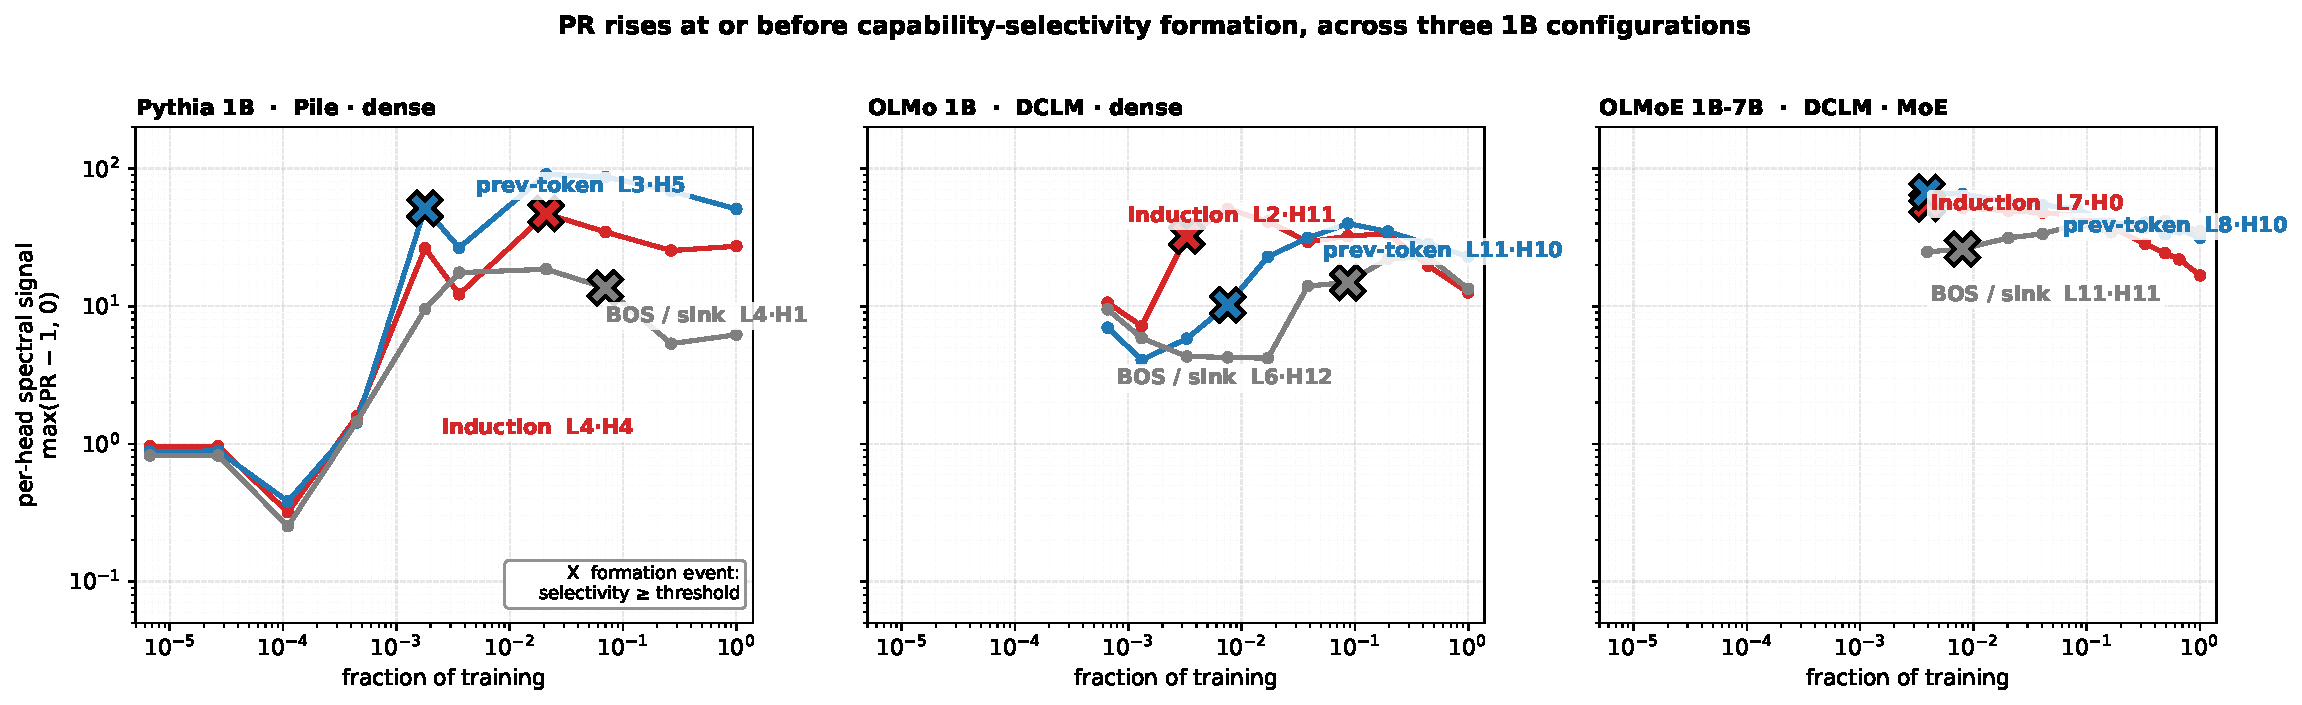
\includegraphics[width=0.98\linewidth]{figures/developmental_three_panel.pdf}
\caption{\textbf{PR rises at or before capability-selectivity formation,
across three 1B-class configurations.} Per-head spectral signal at each
checkpoint, $\max(\prtxt_t-1,0)$ (the integrand of the PR-integral
ranking statistic, plotted per-checkpoint to preserve temporal structure;
same y-axis as Figure~\ref{fig:headline}A). For each of three 1B-class
configurations --- Pythia 1B (Pile, dense), OLMo 1B (DCLM, dense), and
OLMoE 1B-7B (DCLM, MoE) --- one top-selective head per capability class
is plotted: \textsc{induction} (red), \textsc{previous-token} (blue), and
\textsc{first-token / bos} (grey). Identifiers next to each curve give the
$(L,H)$ coordinates in the respective model. X markers indicate the
formation event --- the first checkpoint at which that head's
capability-selectivity ratio exceeds its threshold ($\ge\!50\times$ for
induction, $\ge\!100\times$ for previous-token, $\ge\!30\times$ for
first-token). In every panel and every curve the spectral signal is
elevated at or before the formation event. Lead times on this
10-checkpoint log-spaced grid: induction heads lead by 1--2 checkpoints
across all three models; previous-token heads co-emerge with their
capability selectivity (lead = 0); BOS-attractor heads lead by 2--4
checkpoints (longest in Pythia 1B and OLMoE, shortest in OLMo 1B where
the BOS-attractor transition is sharp; see Section~\ref{sec:f2}). The
cross-configuration consistency of the qualitative claim (PR elevated
at or before formation) is what the figure surfaces; the specific
lead-time numbers vary with the data, architecture, and the granularity
of the checkpoint grid. The empty space at the left of the OLMo and
OLMoE panels reflects the HuggingFace checkpoint-publication limit
discussed in Section~\ref{sec:setup}, not the absence of an underlying
trajectory; the x-axis range is kept uniform across panels for fair
visual comparison.}
\label{fig:dev3}
\end{figure}

\paragraph{Important scope statement.} The claim ``PR rises before
capability selectivity'' holds \emph{for the heads that end up
capability-selective}. It is \emph{not} the same as the claim that
ranking heads by the PR integral $I(L,H)$ identifies capability-specific
heads. In the attention-sink-dominated 1B regime documented in
Sections~\ref{sec:f1}--\ref{sec:f2}, the top-$K$ heads by PR-integral
include L0/L1 generic content-dependent heads and BOS-class heads ahead
of the induction circuit, simply because the BOS-class heads have higher
\emph{sustained} PR through training. PR-integral is a general indicator
of specialized computation; the capability-specific screen of
Section~\ref{sec:method} disambiguates which specialization each head
is doing. We state this scope explicitly here rather than burying it
because it is the most common misreading of the headline figure: the
two-step pipeline (PR-integral $+$ class-specific screen) is necessary
for capability-specific identification in 1B+ models, even though the
PR signal alone is sufficient to flag the heads in
attention-sink-free smaller models.

\section{Discussion}
\label{sec:discussion}

\subsection{The ``induction phase transition'' framing}

\citet{olsson2022} described the formation of induction heads as a sharp
phase transition co-located with a bump in the loss curve and the
emergence of in-context learning. The headline result of this paper is
that, at 1B scale and on DCLM data, the induction transition and the
attention-sink transition are \emph{separated by 10--20$\times$ in
tokens}. The induction circuit reaches its final size at 20--23B tokens
in both DCLM models; the BOS-attractor reaches its 50\% milestone at
264B (OLMo) and 419B (OLMoE). These are not the same training-time event,
even on the same data, and even at adjacent scales (1B active parameters
in both DCLM models).

Three implications follow. First, ``the induction phase transition'' as a
phrase is ambiguous: it can mean the induction-circuit formation event
(20B tokens on DCLM, $\sim$6B on Pile in our panel) or the BOS-attractor
phase transition (264B in OLMo, gradual in OLMoE and Pythia). These are
mechanically distinct events with different timings. Second, sharp
phase-transition character is a property of \emph{specific} (data,
architecture) configurations rather than a universal feature of attention
formation: dense $+$ DCLM produces a sharp BOS-attractor transition;
MoE $+$ DCLM produces a gradual ramp on the same data; dense $+$ Pile
produces a gradual ramp on different data. Third, the relevant
mechanistic claim is no longer ``a single transition near loss-curve
feature $X$'' but ``two distinct transitions whose token-resolved timing
and shape depend on data and architecture.''

\subsection{What a theory of attention sinks must explain}

A complete mechanistic account of attention sinks needs to satisfy at
least three observed constraints from our developmental panel:

\begin{enumerate}
\item \textbf{The L0/L1 zero-BOS floor} (Section~\ref{sec:f1}). No
      gradient signal installs BOS-attractor heads at L0 or L1 at any
      point during training, across all three models. This is a property
      of where in the network BOS can do useful work, not a property of
      the data that eventually produces sinks. A theory of sinks needs
      to predict that the first two layers are off-limits for sink
      installation.
\item \textbf{The data-dependent shape} (Section~\ref{sec:f2}, comparing
      Pythia and OLMo). At fixed architecture (dense) and scale (1B),
      DCLM produces a sharper transition and higher saturation than
      Pile. The data does not just change the asymptote; it changes the
      sharpness of the transition. A theory that predicts the asymptote
      from data alone (e.g., from BOS-token frequency in the corpus)
      is insufficient.
\item \textbf{The MoE smoothing-and-reduction effect}
      (Section~\ref{sec:f2}, comparing OLMo and OLMoE). At fixed data
      (DCLM) and scale (1B active parameters), the MoE architecture
      both reduces the asymptotic BOS-class fraction and smooths the
      dynamics from a sharp transition to a gradual ramp. The
      architectural intervention changes two things at once. A theory
      should ideally identify a single underlying mechanism that
      manifests as both reduction and smoothing.
\end{enumerate}

A natural candidate framework that captures (1) is the
``residual-stream null-space'' picture: at L0 the residual stream is one
token's embedding plus position; at L1 the residual stream is L0's
embedding plus the L0 attention output, which by (1) is itself
content-dependent and never sink-routed. Sink heads can only do useful
no-op work once the residual stream carries a token-mix from
$\ge\!2$ prior layers of attention. We do not develop this picture
quantitatively; it is the kind of theory the L0/L1 floor calls for.

\subsection{Bridge to parameter-space emergence}

This paper studies emergence in \emph{activation space}: PR is a
spectral statistic of per-head attention outputs over an evaluation
batch. The capability selectivity ratio is an averaged attention pattern
on the same batch. Both quantities are activation-side, not
weight-side.

A complementary program studies the same emergence event from the
parameter-side. \citet{xu2026sed} tracks low-dimensional optimizer-induced
drift and transverse dynamics through training, and reports
phase-transition-like changes in the parameter-space geometry at
training-token counts that coincide, in their panel, with
capability-emergence events identified by downstream evaluation.
\citet{xu2026lch} examines spectral-edge dynamics of training
trajectories and finds signal--noise geometry signatures at the same
training-token counts. The picture both papers develop is that
parameter-space and activation-space both register the emergence event,
and that the parameter-space signature can be read out without
constructing a task-specific evaluation.

If the two programs are studying the same event, several questions
sharpen. (i) The L0/L1 floor in activation space presumably has a
parameter-space counterpart: L0 and L1 attention matrices should
\emph{not} develop the spectral signature SED associates with
sink-formation in later layers. (ii) The two distinct transitions
(induction vs BOS-attractor) we observe should map to two distinct
parameter-space transitions, with the BOS-attractor transition's sharp
DCLM-dense character visible in OLMo's weight spectrum. (iii) The
predictive 0.3--2\% training-fraction recall in Section~\ref{sec:f4}
should have a parameter-space analogue: SED's spectral statistic at the
same checkpoints should identify the same set of attention heads. None
of these are tested here; they are the empirical questions an integrated
activation-and-parameter-space theory would need to answer.

\subsection{Practical methodological consequences}

Three concrete recommendations follow from the developmental findings:

\begin{enumerate}
\item \textbf{Apply the capability-screen at intermediate checkpoints
      rather than only the final one.} The 67\% recall threshold is
      reached at 0.3--2\% of total training in all three models, so
      most of the circuit is identifiable from a checkpoint two orders
      of magnitude smaller in training-token count than the final
      checkpoint.
\item \textbf{Distinguish ``induction emergence'' from ``attention-sink
      emergence'' in any developmental analysis.} They are not the
      same event in DCLM 1B models. Conflating them confuses what is
      being studied.
\item \textbf{When BOS-class fraction exceeds $\sim$70\%, use the
      all-head capability-specific screen rather than best-class
      ranking.} Best-class ranking surfaces BOS heads ahead of
      capability heads in this regime, which is the wrong filter for
      capability-specific causal claims (see
      Section~\ref{sec:f5}'s scope statement).
\end{enumerate}

\section{Limitations}

\paragraph{Checkpoint resolution.} The 10 log-spaced revisions per model
are the published HuggingFace checkpoints; finer-grained checkpoints would
catch transitions our grid currently lumps together. Pythia 1B in
particular: the 6B-token co-emergence of induction with BOS-10\% may be
two distinct transitions at finer resolution. The OLMo 1B sharp transition
between 117B (BOS-7\%) and 264B (BOS-70\%) similarly is the
between-checkpoint gap on a $\log_2$-spaced grid; the underlying
transition could be sharper or smoother on a $\log_{10}$-spaced grid.

\paragraph{Seed.} Each of the three 1B models is trained once, with a
single random seed; we do not have within-architecture re-pretraining at
this scale (re-pretraining a 1B-class natural-text model is expensive in
compute). The findings should therefore be read as ``what these specific
runs produced,'' not as ``what the (model, data) configuration produces in
expectation.'' At smaller scale, six seeds of TS-51M
\citep{paper1_methodology} show within-architecture variability in which
heads implement a target capability; we cannot rule out a similar
trajectory-shape variability at 1B.

\paragraph{Evaluation batch.} The capability-selectivity ratios are
computed on the synthetic induction batch (random tokens, structured
$A\,B\,\ldots\,A$ pattern). Whether the same trajectory timings hold on
natural-text induction-target positions is an open question. The
final-checkpoint cross-validation in \citet{paper1_methodology} indicates
the synthetic-batch-identified induction circuit is the circuit doing
induction on natural text in OLMoE; we do not repeat that validation
per-revision in this paper because it would require natural-text batches
on every checkpoint.

\paragraph{MoE forward-pass cost.} OLMoE 1B-7B's forward pass involves
top-8 expert routing across 64 experts, which makes per-revision
mech-interp roughly 2$\times$ more expensive than dense OLMo at the same
nominal parameter count. We sampled 8 OLMoE revisions rather than 10 for
this reason. Two missing revisions are below 20B tokens, which is below
the earliest published HuggingFace checkpoint anyway.

\paragraph{Capability classes.} We tracked induction, previous-token,
self, BOS-attractor, duplicate-token, and local. The class taxonomy is
not exhaustive; in particular, no class in this list captures composed
tasks like IOI. The cross-task generalisation of the capability-screen
recipe is the subject of the companion pattern-selectivity paper
\citep{paper3_circuits}.

\section{Conclusion}

Tracking induction, previous-token, and BOS-attractor head emergence at
10 log-spaced revisions in each of three 1B-class language models reveals
that what is sometimes called ``the induction phase transition'' is, on
DCLM data, two transitions: capability-circuit formation by 20--25B
tokens, and attention-sink formation 10--20$\times$ later. The L0/L1
zero-BOS floor holds across all 30 runs; BOS-attractor formation follows
three distinct shapes across the three (data, architecture) configurations;
the capability-specific screen converges to most of the final induction
circuit within $\sim$1\% of training; and the per-head PR signal is
elevated at or before capability-selectivity threshold crossings, for
every final-checkpoint induction head sampled. The picture that emerges
is of \emph{two distinct training-time transitions} whose timing and
shape depend on data and architecture in separable ways, with the L0/L1
zero-BOS floor as a stable architectural constraint underneath both.

\bibliography{refs}

\end{document}
